\section{The Queue Transmission Model}
The Queue Transmission Model (QTM) consists of a network $\Net = (\Qset,\Lset)$, where $\Qset$ is a set of queues and $\Lset$ is a set of lights. A queue is defined by the tuple $(\QMAX{},\QIN{},\QOUT{},\QDELAY{},\Fvec{},\Prvec{},\QPset{})$, where $\Fvec{}$ and $\Prvec{}$ are vectors of maximum flow rates and turn probabilities into connected queues, $\QPset{}$ is the set of phases controlling the queue, and $\QMAX{}$,$\QIN{}$,$\QOUT{}$, and $\QDELAY{}$ are defined in \ref{tab:constants}. Vehicles travel down the length of the queue at the free flow speed and enter into a vertically stacked queue. A light is defined by the tuple $(\CTMIN{}{},\CTMAX{}{},\Pset)$, where $\Pset$ is the set of phases of the light and each phase is defined by the pair $(\PTMIN[]{}{},\PTMAX[]{}{})$, and where $\CTMIN{}{}$,$\CTMAX{}{}$,$\PTMIN[]{}{}$, and $\PTMAX[]{}{}$ are defined in \cref{tab:constants}. Examples of QTM networks are shown in \cref{fig:network3,fig:network6,fig:network9}.



\subsection{LP Formulation}
We have defined a LP formulation for the QTM supporting non-homogeneous $\DT[]$ and a single binary variable per signal phase. The implementation also supports configurable phase and cycle constraints. The model constants are listed in table \ref{tab:constants} and the variables in table \ref{tab:variables}

\begin{table}[t]
\caption{Constants}
\label{tab:constants}
\centering
\begin{tabular}{ll}
\toprule
Constant & Desciption\\ 
\midrule
$\Qn$ & number of queues  \\ [1mm]
$\Ln$ & number of lights\\ [1mm]
$\Pn$ & number of phases of light $\ell$\\[1mm]
$\Nn$ & number of intervals \\ [1mm]
$\DT$ & time duration of interval $n$\\ [1mm]
$\tn$ & elapsed time at interval $n$\\ [1mm]
$\TMAX$ & maximum elapsed time over all intervals ($t^N$)\\ [1mm]
$\QMAX{i}$ & maximum capacity of queue $i$\\ [1mm]
$\QDELAY{i}$ & propagation delay along queue $i$\\[1mm]
$\QIN{i}$ & maximum inflow to queue $i$ from outside the network\\ [1mm]
$\QOUT{i}$ & maximum outflow from queue $i$ to outside the network\\[1mm]
$\FMAX{i}{j}$ & maximum flow from queue $i$ into queue $j$\\[1mm] 
$\FTURN{i}{j}$ & proportion of total flow out from queue $i$ into queue $j$ (turn probability)\\ [1mm]
$\PTMAX{\ell}{k}$ & maximum allowed duration of phase $k$ of light $\ell$\\ [1mm]
$\PTMIN{\ell}{k}$ & minimum allowed duration of phase $k$ of light $\ell$\\ [1mm]
$\CTMAX{\ell}$ & maximum allowed cycle time of light $\ell$\\ [1mm]
$\CTMIN{\ell}$ & minimum allowed cycle time of light $\ell$\\ [1mm]
\bottomrule\\
\end{tabular}
\end{table}

\begin{table}[h]
\caption{Variables}
\label{tab:variables}
\centering
\resizebox{\textwidth}{!}{%
\begin{tabular}{llll}
\toprule
Variable & Type & Range & Description\\ 
\midrule
$\q{i}$ & continuous & $[0,\QMAX{i}]$ & traffic volume of queue $i$ during interval $n$\\[1mm]
$\qout{i}$ & continuous & $[0,\infty)$ & outflow from queue $i$ during interval $n$\\[1mm]
$\qin{i}$ & continuous & $[0,\infty)$ & inflow to queue $i$ during interval $n$\\[1mm]
$\inq{i}$ & continuous & $[0,\QIN{i}]$ & inflow to the network via queue $i$ during interval $n$\\[1mm]
$\outq{i}$ & continuous & $[0,\QOUT{i}]$ & outflow from the network via queue $i$ during interval $n$\\[1mm]
$\f{i}{j}$ & continuous & $[0,\FMAX{i}{j}]$ & flow from queue $i$ into queue $j$ during interval $n$\\[1mm]
$\p{\ell}{k}$ & binary & $\{0,1\}$ & signal phase $k$ of light $\ell$ during interval $n$(1=green)\\[1mm]
$\pd{\ell}{k}$ & continuous & $[0,\PTMAX{\ell}{k}]$ & duration of phase $k$ of light $\ell$ during interval $n$\\[1mm]
\bottomrule\\
\end{tabular}
}
\end{table}

\subsubsection{Network Constraints}
For a set of time intervals over the period $[0,\TMAX]$, where the duration of each interval $n$ is $\DT$, we define a set of variables for each interval and each queue in the network in table \ref{tab:variables} and the associated constants in table \ref{tab:constants}.

First, all the variables in table \ref{tab:variables} are constrained to be $\ge 0$.
Next we constrain the external flows into and out of $q_j$ during interval $n$,
%\begin{linenomath*}
\begin{align}
\inq{i} &\le \QIN{i} \tag{C1}\label{eq:C1}\\        
\outq{i} &\le \QOUT{i} \tag{C2}\label{eq:C2}
\end{align}
%\end{linenomath*}
and the internal flow from $q_j$ to $q_i$,
%\begin{linenomath*}
\begin{align}
\f{i}{j} &\le \FTURN{i}{j} \sum \limits_{k=1}^{\Qn}  \f{i}{k} \tag{C3}\label{eq:C3}
\end{align}
%\end{linenomath*}
where we find the proportion of flow out of queue $i$ turning into queue $j$ by weighting the total flow by the turn probability $\FTURN{i}{j}$, noting that $\sum_k \FTURN{i}{k}=1$. The flow out from queue $i$ is controlled by the set of phases $\QPset{i}$, so we modulate $\f{i}{j}$ by applying the constraint,
\begin{align}
\f{i}{j} \le \FMAX{i}{j} \sum \limits_{\p{\ell}{k} \in \QPset{i}} {\p{\ell}{k}} \tag{C4}\label{eq:C4}
\end{align}
Where $\p{\ell}{k}$ is 1 if the phase is active during interval n, and 0 otherwise. We can then sum the total flows in and out of each queue,
\begin{align}
\qin{i} &= \inq{i} \DT + \sum \limits_{j=1}^{\Qn}  \f{j}{i} \DT   \tag{C5}\label{eq:C5} \\
\qout{i} &= \outq{i} \DT + \sum \limits_{j=1}^{\Qn}  \f{i}{j} \DT \tag{C6}\label{eq:C6}\\
\qout{i} &\le \q{i} \tag{C7}\label{eq:C7}
\end{align}
with the constraint \ref{eq:C7} that the total flow out of queue $i$ during interval $n$ cannot exceed the volume of the queue at the start of that interval.
Now we can perform the update step for queue $i$ over interval $n$,
\begin{align}
\q{i} &= \q[n-1]{i} - \qout[n-1]{i} + (1-\aph{i})\qin[m]{i} + \aph{i} \qin[m+1]{i} \tag{C8}\label{eq:C8}\\
\q{i} &\le \QMAX{i} \tag{C9}\label{eq:C9}\\
(1-\aph{i})\qin[m]{i} + \aph{i} \qin[m+1]{i} + \sum \limits_{k=m+2}^n \qin[k]{i} &\le \QMAX{i} - \q[n-1]{i}\tag{C10}\label{eq:C10}
\end{align}
where $m$ is the interval containing $\tn - \QDELAY{i}$ such that, 
\begin{equation}
\tn[m] \le \tn-\QDELAY{i} < \tn[m+1]
\end{equation}
Since the model is piecewise linear, we linearly interpolate $\qin{i}$ across the interval $m$ to find the inflow to queue $i$ at $\tn - \QDELAY{i}$, and $\aph{i}$ is calculated in a pre-computation step for all $i$ and all $n$,
\begin{align}
\aph{i} &= \frac{\tn - \QDELAY{i} - \tn[m]}{\DT[m]}
\end{align}
Note that if $\QDELAY{i}$ is a homogeneous number of time intervals, $n-m$, then $\tn - \QDELAY{i} - \tn[m]=0$ and constraint \ref{eq:C8} reduces to
\begin{equation}
\q{i} = \q[n-1]{i} - \qout[n-1]{i} + \qin[m]{i}
\end{equation}

\remark{Show diagrams with traffic predictions converging as time increment gets smaller.
  Validates that large time-steps are rough approximations while model behavior converges
for small time steps.}

\begin{figure*}[t!]
\centering
%  trim={<left> <lower> <right> <upper>}
\subfigure[]{
\label{subfig:converg_a}
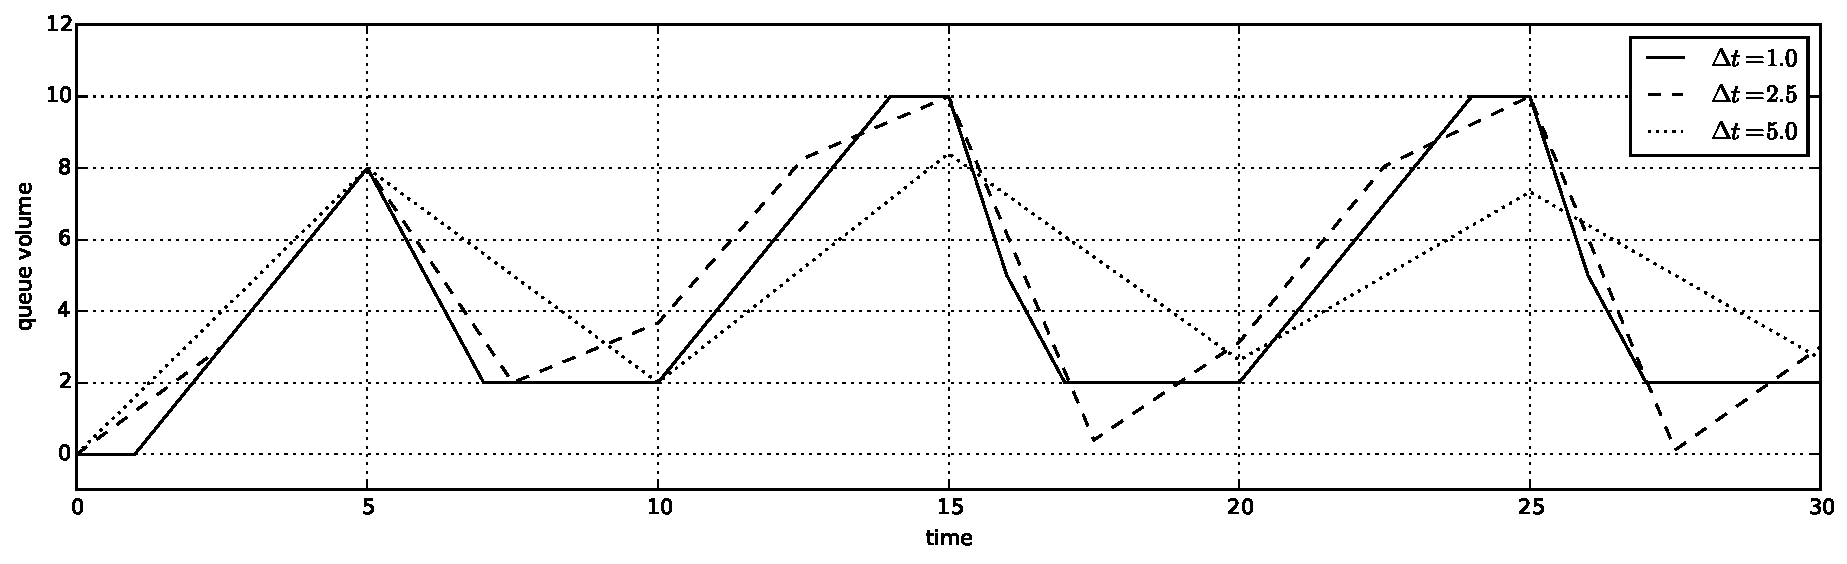
\includegraphics[width=1.0\textwidth,trim={0cm 0cm 0cm 0cm},clip]{convergence.pdf}
}
\subfigure[]{
\label{subfig:converg_b}
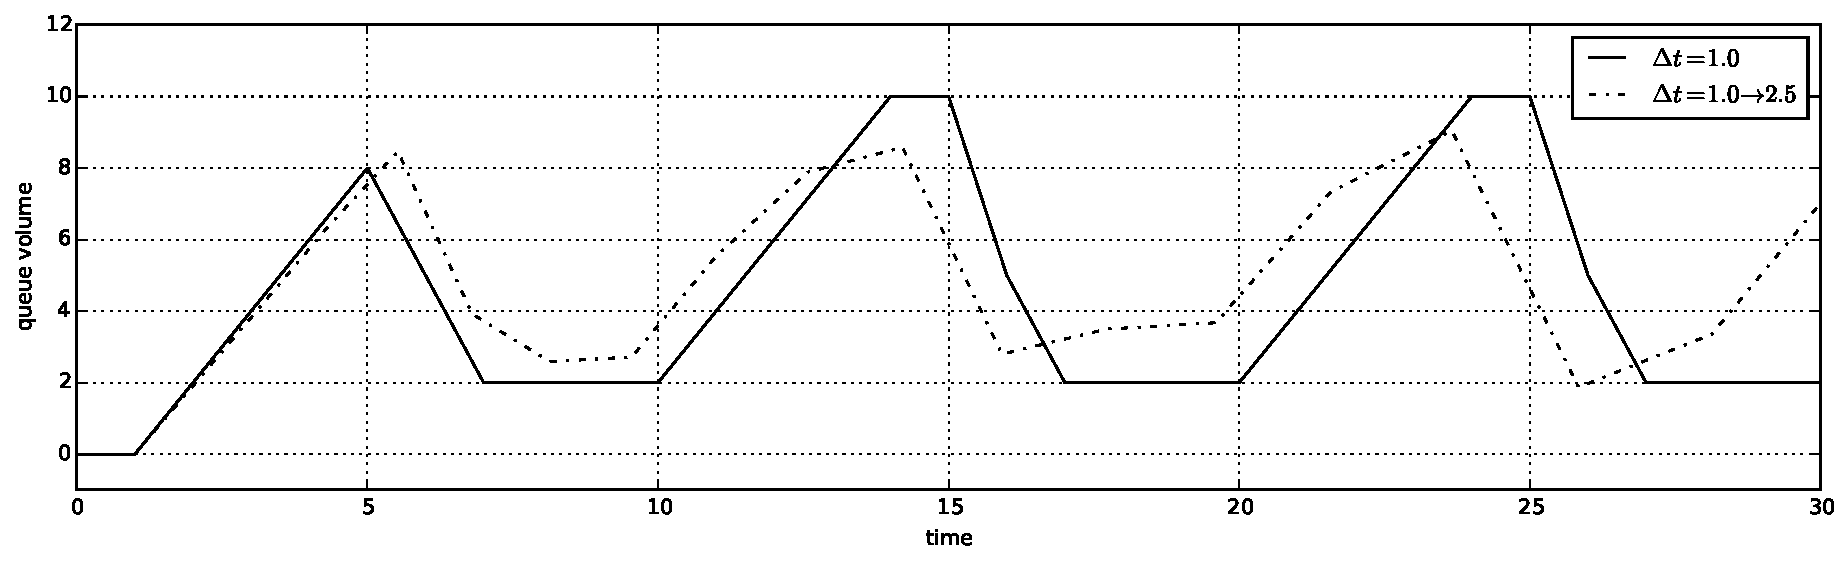
\includegraphics[width=1.0\textwidth,trim={0cm 0cm 0cm 0cm},clip]{convergence_vari.pdf}
}
\caption{An example showing the evolution of traffic volume in a queue over time. (a) Convergce with increasing refinement of $\Delta t$ from $5.0$ down to $1.0$. (b) Dilation of $\Delta t$ from $1.0$ to $2.5$ compared to a fixed $\Delta t$ of $1.0$.}

\end{figure*}

\begin{figure*}[t!]
\centering
%  trim={<left> <lower> <right> <upper>}

\label{subfig:converg_c}
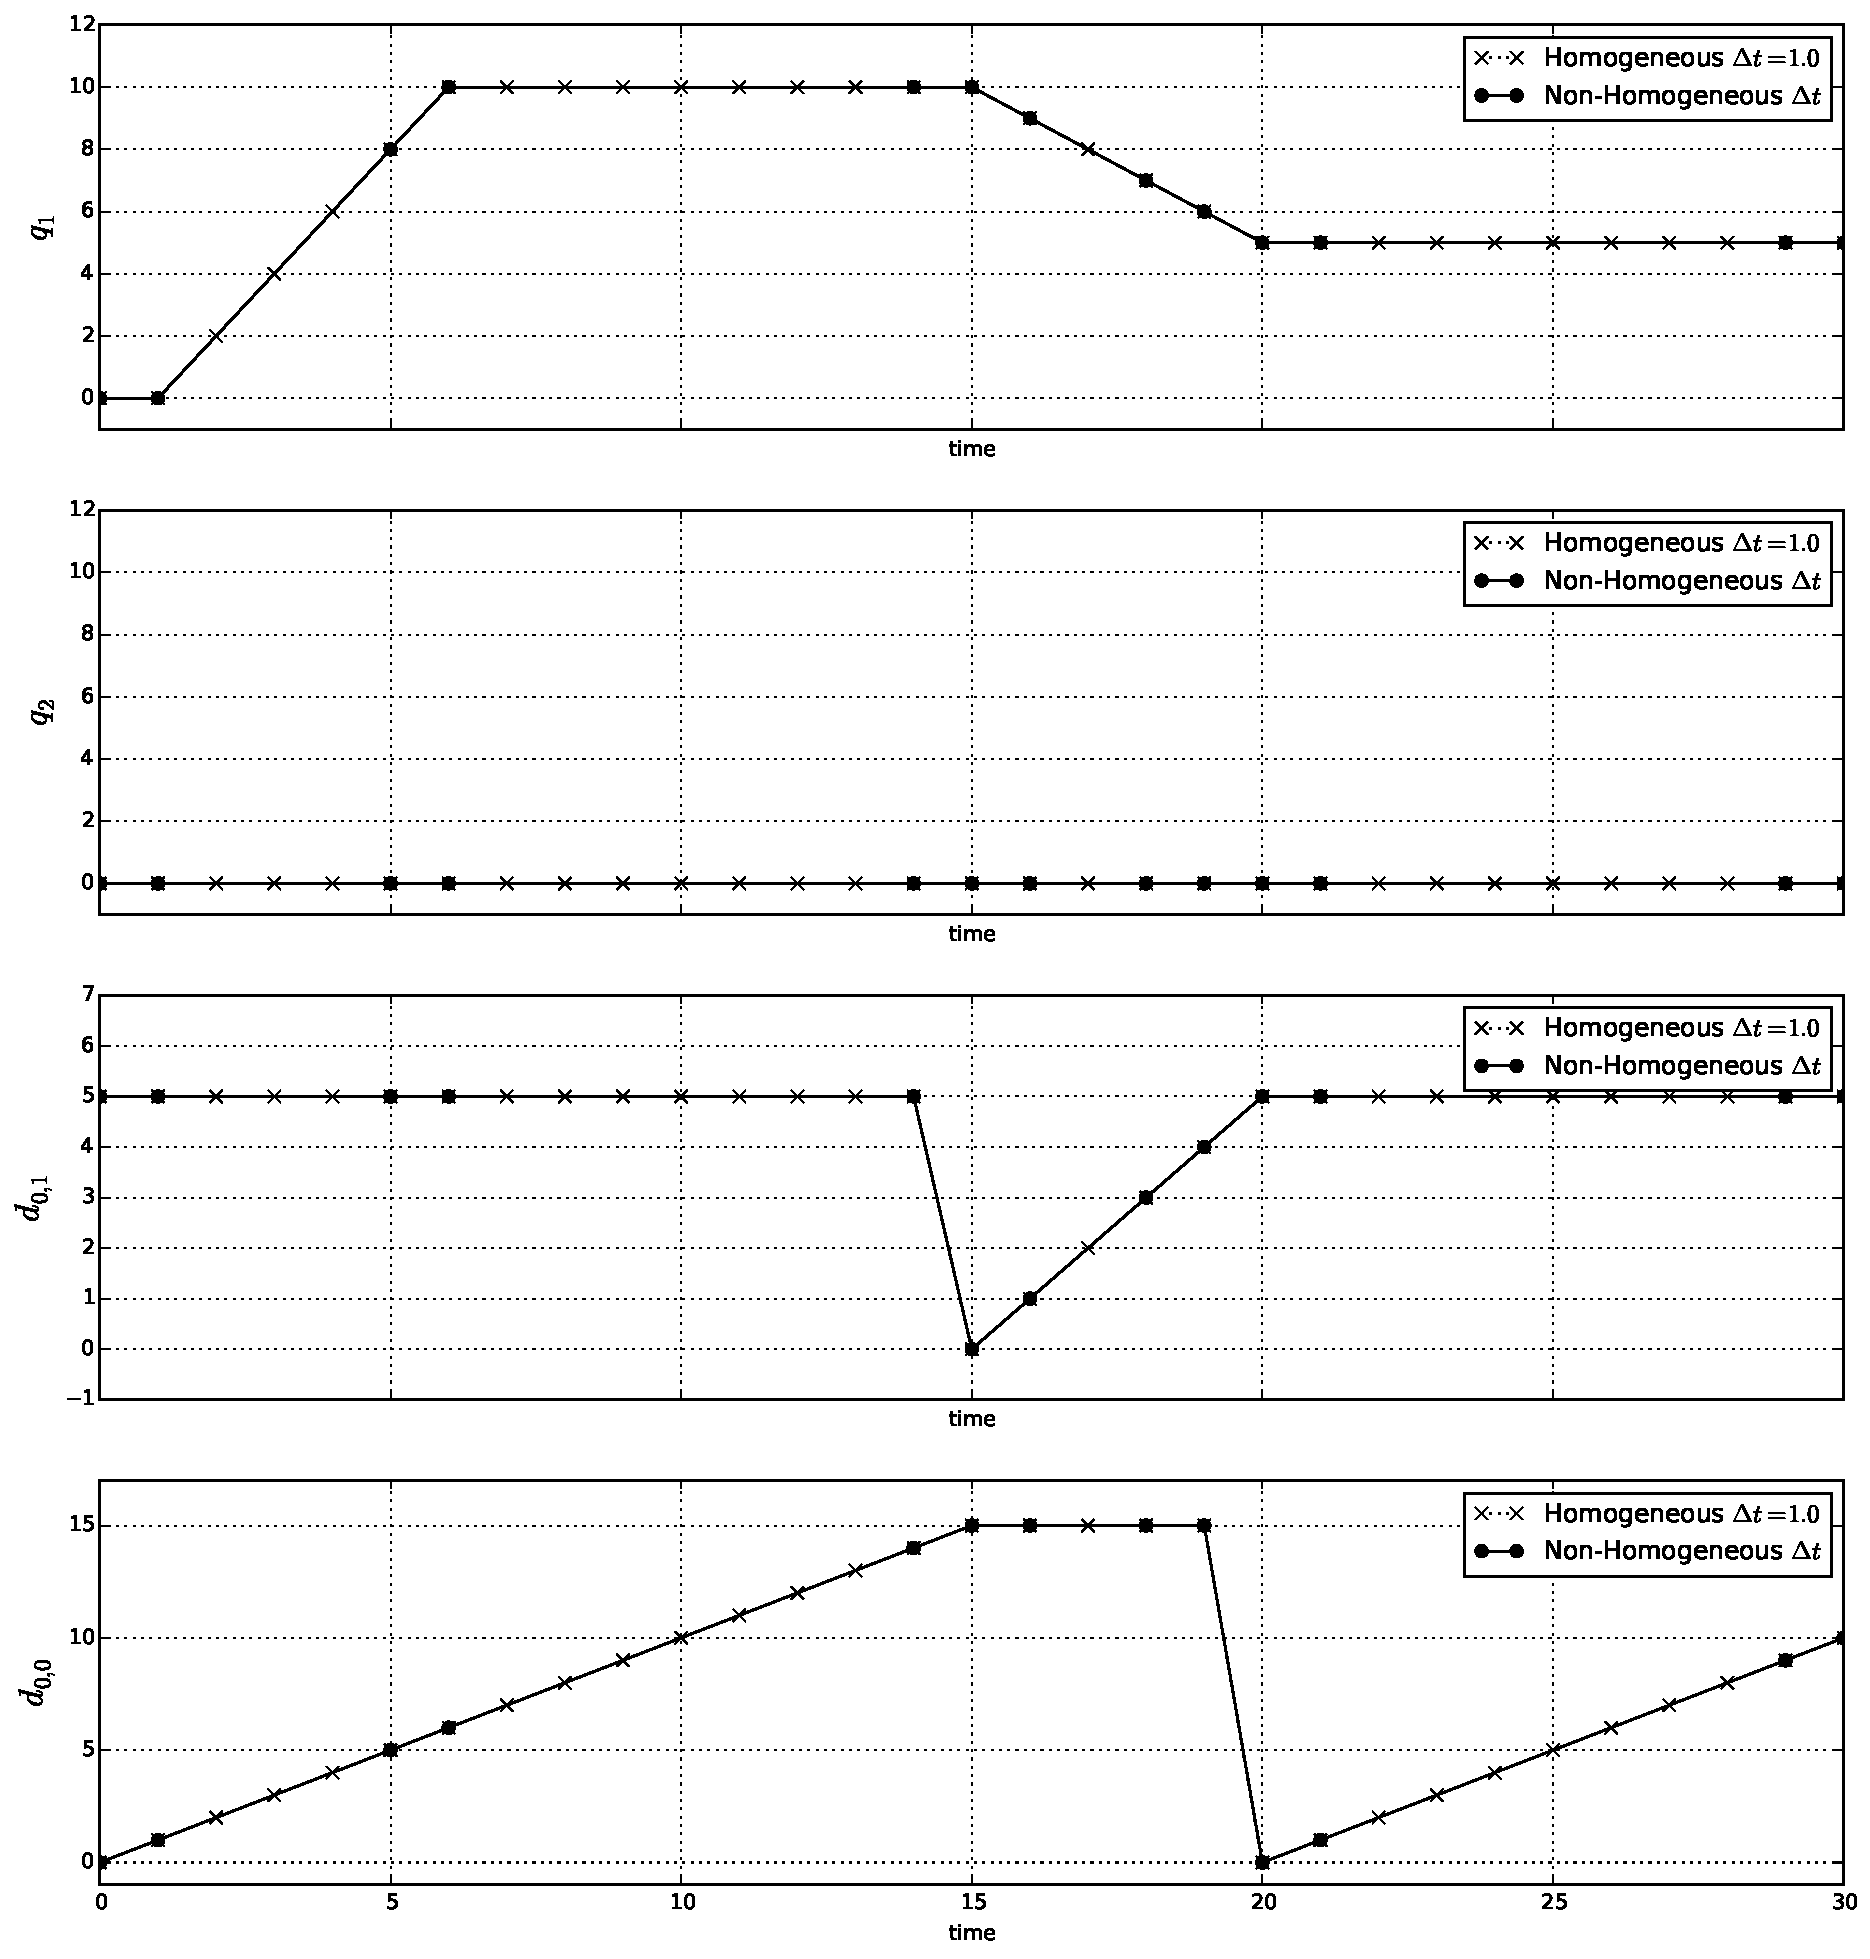
\includegraphics[width=1.0\textwidth,trim={0cm 0cm 0cm 0cm},clip]{convergence_NH.pdf}
\caption{An example showing the convergence between a homogeneous solution with $\Delta t=1.0$ and a non-homogeneous solution over 30 seconds for the same network. By using non-homogeneous time steps the same solution is found with only 14 sample points compared to 30 for homogeneous solution.}

\end{figure*}

\subsection{MILP Formulation}
If we take $p_i^n \in \Pi(0,\TMAX)$, where $\Pi$ is a fixed signal plan over all the intervals from 0 to $T^{MAX}$, then the constraints \ref{eq:C1} to \ref{eq:C10} form a dynamic, piecewise linear model of flow in the network over time as a function of $\Pi$. Alternatively we can define $p_j^n$ as a binary variable and solve to find both a network flow and an optimal signal plan for a given objective function.

\subsubsection{Phase constraints}
First we map each $p_i^n$ to a signal phase $k$ of a light $\ell$ as $\p{\ell}{k}$ (Note that there could be more than one queue mapped to each $\p[]{\ell}{k}$, or their could be none). Then we define a set of constraints for the signal phases. For each traffic light $\ell$, we constrain the phases of $\ell$ such that exactly one phase is active in each interval $n$, and so that they activate sequentially,
\begin{align}
\sum\limits_{k=1}^{\Pn} \p{\ell}{k} &= 1\tag{C11}\label{eq:C11}\\
\p{\ell}{k} + \p{\ell}{k+1} &\le 1\tag{C12}\label{eq:C12}\\
\p[n-1]{\ell}{k} &\le \p{\ell}{k} + \p{\ell}{k+1}\tag{C13}\label{eq:C13}
\end{align}
where $k+1=1$ if $k=P_l$. The constraints \ref{eq:C12} and \ref{eq:C13} ensure that if $\p[]{\ell}{k}$ was active during interval $n-1$ and has become inactive in interval $n$, then $p_{l,k+1}$ becomes active in interval $n$.

Next we enforce the minimum and maximum phase durations, $\PTMIN{\ell}{k}$ and $\PTMAX{\ell}{k}$ for each $\p[]{\ell}{k}$, by defining a duration variable $\pd[]{\ell}{k}$ for each phase. When $\p[]{\ell}{k}$ is active, $\pd[]{\ell}{k}$ holds the elapsed time since the start of phase $k$, and when phase $k$ is inactive $\pd{\ell}{k}$ is constant and holds the duration of the last phase until the next activation,
\begin{equation}
\pd{\ell}{k} = 
\begin{cases}
\pd[n-1]{\ell}{k} + \DT[n-1] & \p[n-1]{\ell}{k}=1,\p{\ell}{k}=1\\
\pd[n-1]{\ell}{k} & \p{\ell}{k}=0\\
0 & \p[n-1]{\ell}{k}=0,\p{\ell}{k}=1
\end{cases}
\end{equation}

We achieve this by applying a set of linear envelope constraints, using the ``big M'' trick to activate each section of the envelope depending on the state of $\p[]{\ell}{k}$, where ``big M'' can be limited to $\PTMAX{\ell}{k}$.
\begin{align}
\pd{\ell}{k} &\le \pd[n-1]{\ell}{k} + \DT[n-1] \p[n-1]{\ell}{k} + \PTMAX{\ell}{k} (1 - \p[n-1]{\ell}{k})\tag{C14}\label{eq:C14}\\
\pd{\ell}{k} &\ge \pd[n-1]{\ell}{k} + \DT[n-1] \p[n-1]{\ell}{k} - \PTMAX{\ell}{k} (1 - \p[n-1]{\ell}{k})\tag{C15}\label{eq:C15}\\
\pd{\ell}{k} &\le \pd[n-1]{\ell}{k} + \PTMAX{\ell}{k} \p[n-1]{\ell}{k}\tag{C16}\label{eq:C16}\\
\pd{\ell}{k} &\ge \pd[n-1]{\ell}{k} - \PTMAX{\ell}{k} \p{\ell}{k}\tag{C17}\label{eq:C17}\\
\pd{\ell}{k} &\le \PTMAX{\ell}{k}(1 - \p{\ell}{k} + \p[n-1]{\ell}{k})\tag{C18}\label{eq:C18}
\end{align}
Then we constrain the phase duration to be between $\PTMIN{\ell}{k}$ and $\PTMAX{\ell}{k}$,
\begin{align}
\pd{\ell}{k} &\le \PTMAX{\ell}{k}\tag{C19}\label{eq:C19}\\
\pd{\ell}{k} &\ge \PTMIN{\ell}{k}(1 - \p{\ell}{k})\tag{C20}\label{eq:C20}
\end{align}
Finally, we constrain the sum of all the phase durations for light $\ell$ to be within the cycle time limits $\CTMIN{\ell}$ and $\CTMAX{\ell}$,
\begin{align}
\pd[n-1]{\ell}{1} + \sum\limits_{k=2}^{\Pn} \pd{\ell}{k} &\le \CTMAX{\ell} \tag{C21}\label{eq:C21}\\
\pd[n-1]{\ell}{1} + \sum\limits_{k=2}^{\Pn} \pd{\ell}{k} &\ge \CTMIN{\ell} (\p{k}{1} - \p[n-1]{k}{1})\tag{C22}\label{eq:C22}
\end{align}
Note, that in \ref{eq:C21} and \ref{eq:C22} we use the duration of phase 1 from the previous interval, $n-1$,  since when we arrive at the beginning of the next cycle of light $\ell$ and the phase sequence starts again from phase 1, $\pd{\ell}{1}=0$ and $\pd[n-1]{\ell}{1}$ is set to the duration of the previous activation of phase 1, and we can sum the total duration of the last cycle across all the phases. Additionally in \ref{eq:C22} we activate the minimum cycle time constraint at exactly the beginning of the cycle with the signal $\p{k}{1} - \p[n-1]{k}{1}$. This is illustrated in figure \ref{fig:phase_plots}(d).

\begin{figure*}[t!]
\centering
%  trim={<left> <lower> <right> <upper>}
\subfigure[]{
\label{subfig:test1}
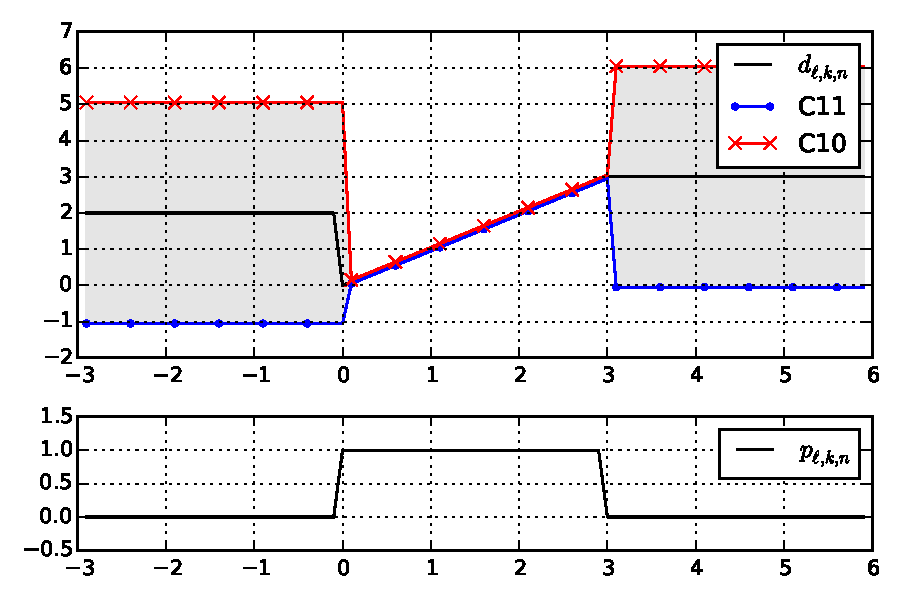
\includegraphics[width=0.45\textwidth,trim={0cm 0cm 0cm 0cm},clip]{phase_plot_fig_1.pdf}}
\subfigure[]{
\label{subfig:test2}
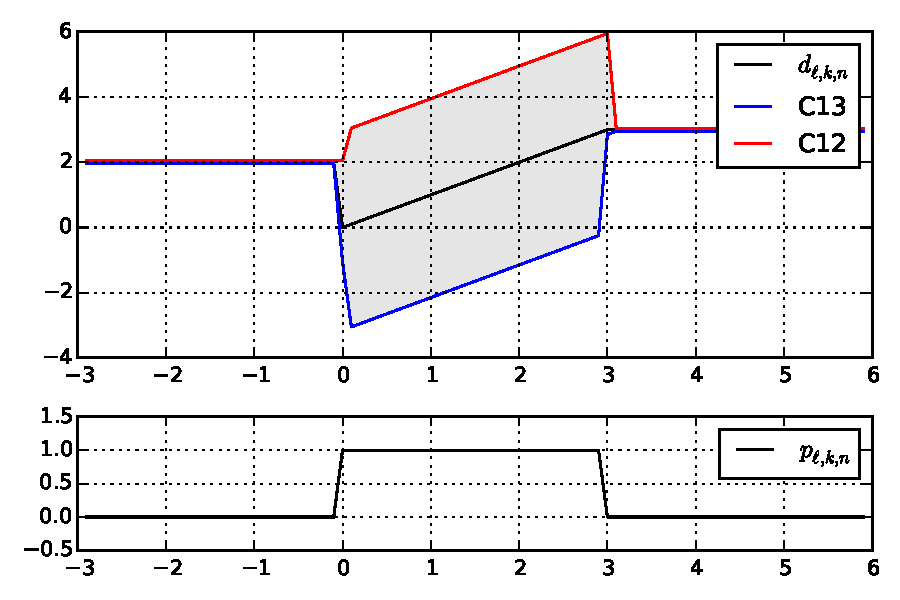
\includegraphics[width=0.45\textwidth,trim={0cm 0cm 0cm 0cm},clip]{phase_plot_fig_2.pdf}}
\subfigure[]{
\label{subfig:test3}
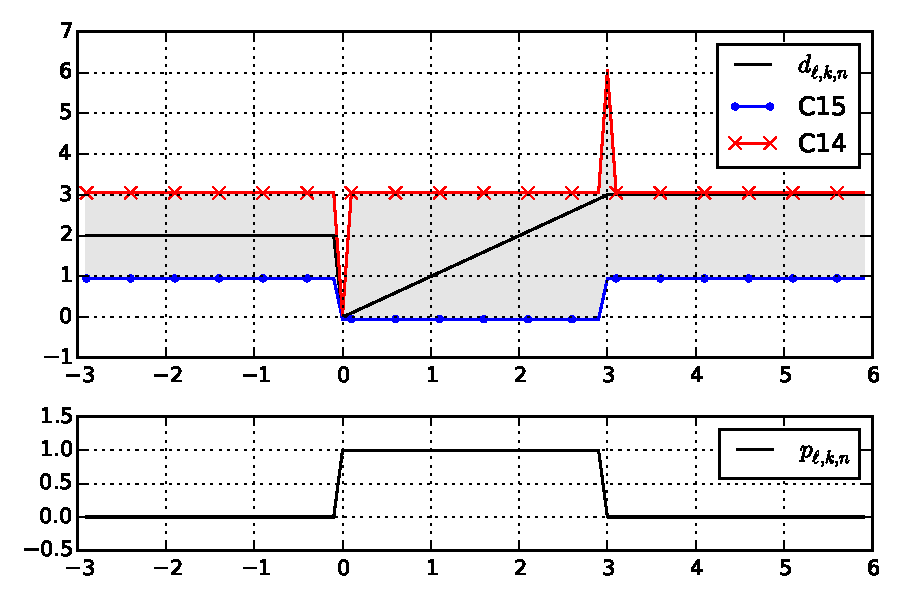
\includegraphics[width=0.45\textwidth,trim={0cm 0cm 0cm 0cm},clip]{phase_plot_fig_3.pdf}}
\subfigure[]{
\label{subfig:test4}
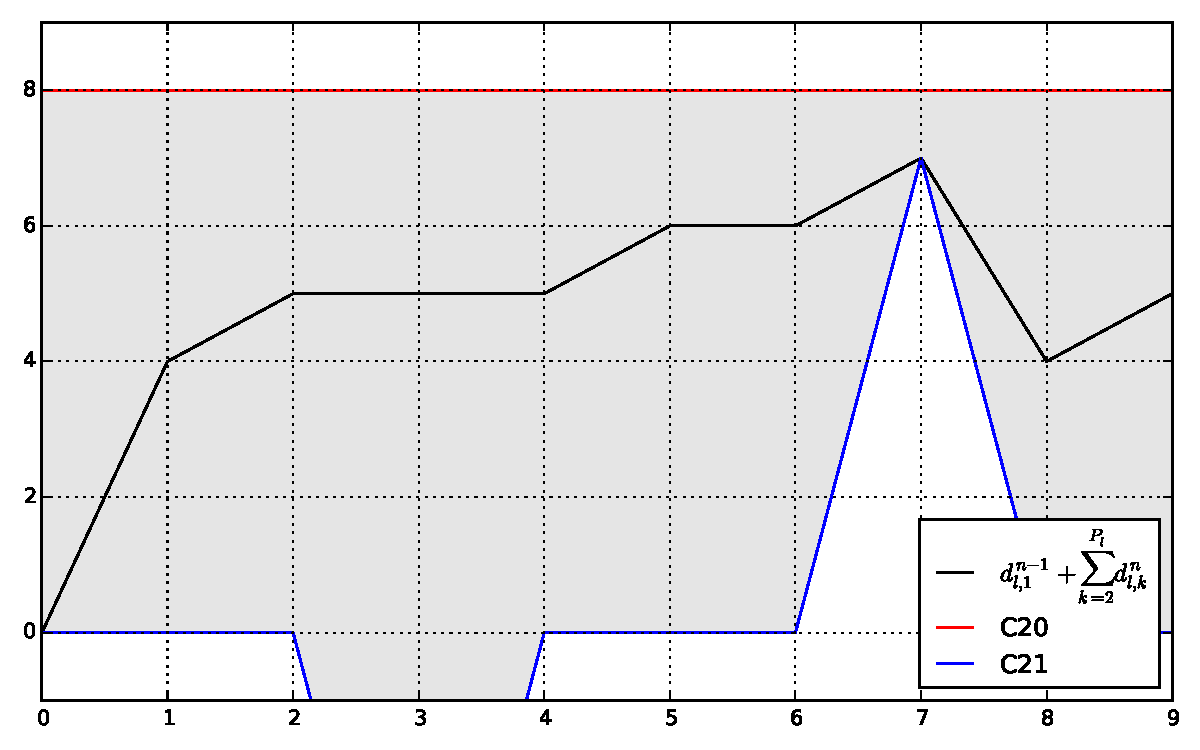
\includegraphics[width=0.45\textwidth,trim={0cm 0cm 0cm 0cm},clip]{phase_plot_fig_4.pdf}}
\caption{An example showing the phase and cycle time constraint envelopes. In (a), (b) and (c), $\PTMIN{\ell}{k}=1$ and $\PTMAX{\ell}{k}=3$, the duration of the previous activation was 2 and the duration of the current activation is 3. In (d), the total cycle time is 7 with $\CTMIN{\ell}=7$, $\CTMAX{\ell}=8$}
\label{fig:phase_plots}
\end{figure*}

\subsection{Objective Function}
\trbcite{lin2004enhanced} derive an objective function for the minimisation of total delay based on the difference between the cumulative departure and arrival curves at the origin and destination. However, such an approach requires the network to be cleared at the end of the optimisation period. We derive an objective function for the maximisation of flow in the network, and apply it to every queue in the network at $\qout{i}$,
\begin{equation}
\textrm{maximise} \left( \sum\limits_{n=1}^{\Nn} \sum\limits_{i=1}^{\Qn} (\TMAX - \tn + 1) \qout{i} + \sum\limits_{n=1}^{\Nn} \sum\limits_{i=1}^{\Qn} (\TMAX - \tn + 1) \inq{i} \right) 
\tag{O1}\label{eq:O1}
\end{equation}
And with the addition of the second $\inq[]{i}$ term, \ref{eq:O1} also ensures that \ref{eq:C1}, \ref{eq:C2}, and \ref{eq:C4} are also at their maximum upper bound.

\remark{It is explanatory here to show the inflow/outflow and delay curves and explain graphically what is going on and how this objective relates.}
